\lhead{\emph{AMC Prototype Feedback and Control Algorithm}}

\chapter{AMC Prototype Feedback and Control Algorithm}\label{ch:operation}

% In Chapter~\ref{ch:amcP}, the overall system has been described.  Each component of the system was discussed in detail.

% This chapter is about
% \begin{itemize}
%     \item how the system works as a unit to provide magnetic field control.  This includes the algorithm which generates the control and some typical results from its operation.  It also includes the methods used in operating the system, such as methods used in tuning the PI control system.
%     \item simulation methods used to understand system performance, and some basic results from the simulation which are compared with data
%     \item definition of metrics that will be used to quantify further system performance.  These will be applied in Chapter~\ref{ch:quantification} where further results will be presented.
% \end{itemize}



% Much of this work follows the work of others, especially Refs.~\cite{bea,rawlik,lins}.  New work that builds on these results is presented in Chapter~\ref{ch:quantification}.

%This chapter describes the main tool that generates the required currents that should be fed to the coils for compensation.
%The algorithm is based on the control theory and similar to as discussed in Ref. \cite{bea}.

% Simulation methods used to understand the system performance are compared with the data
This chapter describes how the system works as a unit to provide magnetic field control. The description includes the algorithm which generates the feedback and control mechanism and some typical results from operation.  It also includes the methods used in operating the system, such as tuning methods used in the control algorithm. Finally, metrics are defined that will be used to further quantify the system performance. These will be applied in Chapter~\ref{ch:quantification} where more results and solutions to problem encountered in the operation of the system will be presented. Much of the work presented in Chapter~\ref{ch:operation} follows the work of others, especially Refs.~\cite{bea,rawlik,lins}.  New work that builds on these results is presented in Chapter~\ref{ch:quantification}.

\section{Principle of Operation\label{sec:process}}

% The goal of this Section is to tell the general idea of how the system works, and to introduce the principles of operation.  It also introduces a few of the key issues faced when operating the system.

% \begin{itemize}
%     \item fluxgates (hopefully described in some Section in Chapter~\ref{ch:amcP}) measure the field
%     \item a setpoint for each fluxgate axis is decided
%     \item when the fluxgate signal drifts from the setpoint, the error grows
%     \item how the fluxgates respond to changes in the current is described by a matrix
%     \item the inverse of the matrix describes how to correct the currents based on fluxgate signals
%     \item PI control is used to decide the corrected currents based on the input errors from the fluxgate readings
% \end{itemize}

% Details:
% \begin{itemize}
%     \item the matrix isn't square and its inverse has to be defined
%     \item the problem can be ill-conditioned so that the matrix must be regularized in order that small changes in currents do not generate large, uncontrolled fluctuations in field.  The regularization itself is nontrivial.
%     \item the PI loop must be tuned
% \end{itemize}


% \fig{Images/feedback}{width = 0.6\textwidth}{PI loop in flow chart.\label{fig: feedback}}
% The first measurement from the sensors after filtering (see section \ref{sec:f}) will act as setpoint ($B_{setpoint}$)


% The basic idea is that there will be a goal/setpoint with whom the consecutive measurement will be compared and any deviation from the setpoint will be minimized by the Proportional Integral (PI) feedback algorithm. For this prototype, the first measurement from the sensors after filtering (see section \ref{sec:filter}) will act as setpoint. Then the repeated measurements from the sensors have been taken. For each measurement, difference with the setpoint is  noted as -
% \begin{equation*}
%     \Delta B = B(setpoint) - B(measure)
% \end{equation*}
% % The current is related to magnetic field by- 
% % \begin{equation*}
% %     B=M \times I
% % \end{equation*}
% % Where, $\bm{M}$ is the matrix of proportionality factor in $nT/A$. So, the difference in current can easily be found by -
% % \begin{equation*}
% %     \Delta I=M^{-1} \times \Delta B
% % \end{equation*}
% On the basis of that, PI feedback algorithm will generate the required current that should be fed to the coils to compensate $\Delta B$. After certain period, a perturbation is also applied using an eletro-magnet coil to test how good the system is performing.  The above process is repeated as long as the compensation is running. 

The goal of this Section is to tell the general idea of how the feedback system works, and to introduce the principles of operation.  It also introduces a few of the key issues faced when operating the system. 

Fluxgates measure the magnetic field. Each fluxgate axis has a setpoint. When the fluxgate signal drifts from the setpoint, the error grows. The fluxgates respond to changes in the coil currentsin a linear fashion and can therefore be described by a matrix. The inverse matrix describes how to correct the currents based on the errors from the consecutive fluxgate signals. A Proportional Integral (PI) control algorithm  is used in conjunction with the matrix inverse to correct currents based on the error signals. The matrix isn't square and its inverse has to be defined. A problem arises that the matrix can be ill-conditioned, and this problem must be dealt with. 

In the upcoming Sections, the mathematical definitions required to explain system operation will be discussed. Issues encountered in ill-conditioning and the mathematical principles of non-square matrix inversion will be covered and some basic results of the measurements after tuning the PI parameters will be shown. Metrics of the system performance are also discussed. Chapter~\ref{ch:quantification} relates to use of these tools to characterize system performance, focusing on the novel aspects of any work.

\section{Matrix of Proportionality Factors}\label{sec:m}
% where subscript indices $s$, $c$ and $n$ has been used to indicate sensors, coil and no. of measurement respectively.
% The matrix relates the currents in the six coils to the magnetic field readings in the 12 sensors.
As previously discussed in Sections~\ref{sec:cube} and~\ref{sec:sensor}, there are total 14 sensor axes and 7 coils for the prototype. Among them, 12 sensors and 6 coils are used for compensation and others are used for quantification. The magnetic field readings change linearly with current, represented by a constant matrix $\bm{M}$. The matrix is a constant if we ignore hysteresis. This is generally a good approximation because the magnetic permeability of the nearby magnetic shields is very large.

\begin{table} [htb!]
    \centering
    \begin{tabular} { |c|c|c|c|c|c|} 
        \hline
        Index & Range & Labels & Definition\\
        \hline\hline
        $c$ & 1-6  & $C_x^\pm$, $C_y^\pm$ and $C_z^\pm$  & Define specific coil \\ 
        \hline
        $S$ & 1-14  & \makecell{1$x$, 1$y$, 1$z$ or \\3$x$, 3$y$, 3$z$ or\\ center-$x$ ... center-$z$ \\ etc. (see Fig.~\ref{fig:coil})}  & \makecell{Define the $x$, $y$ and $z$ \\of a specific position \\ (Numbering based \\on positions). \\Control sensors used\\ on the center\\ of the prototype} \\ 
        \hline
        $s$ & 1-12  & \makecell{Same as labels of $S$}  & \makecell{Subset of $S$ excluding\\ the 2 control sensors} \\ 
        \hline
        $n$ &  0$<N<\infty$ & 1,2,3,..,$N$  & \makecell{Define no. of \\PI loop iterations} \\ 
        \hline        
    \end{tabular}
    % \vspace{4mm}
    \caption[Definition of different indices used to indicate sensor, coil and iterations]{Definition of different indices used to indicate sensor, coil and iterations in the feedback loop. Each sensor and coil also has a label which identifies it physically.}\label{table:index}
\end{table}

The relationship between the relative sensor readings and the coil currents is
\begin{equation}\label{eq:B_coils}
    B_s^n(\mathrm{coils})=\sum_{c=1}^{6} M_{sc} I_c^n
\end{equation}
where, $M_{sc}$ are the elements of the matrix $\bm{M}$ and $I_c^n$ is the current set on the coils for a particular measurements where $n$ runs from 0 to $N$ for $N$ being total number of measurements. The sum is over coils $c$ and the sensor index $s$ runs from 1 to 12. They are defined in Table~\ref{table:index}. The field $B_s^n(\mathrm{coils})$ refers only to the relative field, in the sense that it is the field generated at sensor $s$ by the coil set. There could be other fields from the environment, which are the fields we seek ultimately to correct as will be discussed in the following Section~\ref{sec:pi}.




%\FloatBarrier


The matrix defined in this way is easy to measure using the system.  Each coil $c$ is set to a current, with all other currents set to zero.  The change in the sensor reading $s$ then gives the matrix element $M_{sc}$. 


\fig{Images/Mdiff3_31}{width =0.9\textwidth}{Color map of $\bm{M}$ measured using the scheme indicated in the text.  Horizontal axis indicates the various sensors, which are counted using the index $s$.  Vertical axis indicates the various coils, which are counted using the index $c$.  The color axis ($z$-axis) indicates the value of the matrix element.  Red elements indicate positive values while blue elements indicate negative values.  Elements that appear white are near zero in the matrix element.\label{fig:m}}{Color map of $\bm{M}$}

%\FloatBarrier
The color map of a matrix $\bm{M}$ measured in this fashion is shown in Fig.~\ref{fig:m}.  The results are reasonable considering the design of the system.  The system was designed to compensate magnetic field of order 100~nT for currents of 200~mA, which would imply the matrix elements should be of scale 500~nT/A.  Generally this agrees with the color scale seen in Fig.~\ref{fig:m}.  Furthermore, the strongest matrix elements are those where the coil is closest to the sensor in question.  For example, 8y is closest to coils Y- and X+.  It also makes sense that 8y would have strong matrix elements here because it is near the corner of the magnetic shield which causes {\it e.g.} the X+ coil to be converted into a strong y component.  The red and blue colors are a result of the definitions of positive/negative current in relation to coil in question's orientation and the sensor axis definition.



\section{Implementation of PI Control Algorithm}\label{sec:pi}
 In my algorithm, the magnetic field is measured using the fluxgates and used to define the setpoints. As will be shown, when the field changes, the error in the field can be translated into an error in current based on inverting Eq.~(\ref{eq:B_coils}). New current values are then calculated that must be fed to the coils completing the PI control loop. 

% The measurement from the fluxgate sensors will have  the contribution from both the environment and  the field generated at sensors by the coil set of specific current value as presented in Eq.~(\ref{eq:B_coils} and can be related by 
% \begin{equation}\label{eq:B}
%     B_s^n (measure) = B_s^n(environment)+ B_s^n(coils)
% \end{equation}

The typical magnetic field of the surroundings has been measured using a fluxgate and is reported in Table~\ref{table:Benvironment}. The values are similar in scale to Earth's magnetic field which is $\sim$42 $\mu$T in vertical downward direction. These are the typical scale of the setpoints.

\begin{table} 
    \centering
    \begin{tabular} { |c|c|c|c|c|c|} 
        \hline
        Axis & \makecell{Typical B field \\($\mu$ T)}\\
        \hline\hline
        $x$ & 10 \\ 
        \hline
        $y$ & 42 \\ 
        \hline
        $z$ & -5 \\ 
        \hline
    \end{tabular}
    % \vspace{4mm}
    \caption[Typical magnetic fields surrounding the prototype]{Typical magnetic field values of the environment surrounding the prototype obtained from fluxgate measurements when the $x$, $y$ and $z$ axis represent the northward, vertical downward, and westward direction respectively. }\label{table:Benvironment}
\end{table}

%\FloatBarrier
For PI control, the setpoint is measured using the fluxgate array by applying 100 mA current to the coils. Our current sink (see Section~\ref{sec:sink}) can generate 0-200 mA current. So, the 100 mA current has been chosen to utilize the full capacity of the current sink to compensate the field fluctuations in either direction. After finding the setpoint from the first measurement of the fluxgates, the change in the fluxgate signal is
\begin{equation}\label{eq:del_B}
    \Delta B_s^n = B_s(\mathrm{setpoint}) - B_s^n(\mathrm{measure})
\end{equation}

For iteration $n=1$, Eq~(\ref{eq:del_B}) will give zero value as the first measurement is acting as to be setpoint, as explained earlier. The consecutive measurements are used in the control algorithm. 

Using the relationship between the sensor readings and the coil currents as explained in Eq.~(\ref{eq:B_coils}) and the $\Delta B_s^n$ obtained from Eq.~(\ref{eq:del_B}), the error in terms of the current  will be
\begin{equation}\label{eq:del_I}
    \Delta I_c^n =\sum_{s=1}^{12} M^{-1}_{cs} \Delta B_s^n~\text{.}
\end{equation}
Here, $M^{-1}_{cs}$ are the elements of the inverse of the matrix $\bm{M}$. The inversion of the non-square matrix is a subtle problem and is discussed in Section~\ref{sec:inv}. $\Delta I_c^n$ is the error for $n^{\mathrm{th}}$ measurement on the basis of which the new set of currents will be calculated using a PI control algorithm. That is, the control variables in our case are the currents in the coils. The errors are also currents, those deduced from matrix inversion and magnetic sensor deviations from setpoints. In the algorithm, the new current~\cite{bea} is
\begin{equation}\label{eq:I}
    I^n_c=I^0_c+k^p_c \Delta I_c^n+k^i_c\sum_n \Delta I_c^n
\end{equation}
where, $I^0_c$ indicates the initial value of current for the set of the coils when the setpoint has been set (100 mA). $\Delta I_c^n$ is the error found using Eq.~(\ref{eq:del_I}) and the sum is over iterations $n$. The term $k^p_c$ is the proportional gain (P) and $k^i_c$ is the integral reset (I) for a particular coil. The gains $k^p_c$ and $k^i_c$ terms need to be tuned properly as will be explained in Section~\ref{sec:tune}. The index $c$ in $k^p_c$ and $k^i_c$ terms represents that the P and I value for for each coil could in principle be different. But throughout the thesis, I have used same values of $k_c^p$ and $k_c^i$ in all six coils. We found derivative term (D) in a typical PID scheme was unnecessary because it relates to optimizing fast response and our chief concern is long-term stability.

\fig{Images/1s1c1zc1}{width =0.9\textwidth}{The $C_x^-$ coil current (left) and magnetic field $\Delta B$ (right) for sensor 1z with $k_c^p=1.0$, and $k_c^i=0.0$. Green curve:  measured field.  Red curve: predicted uncompensated field (Eq.~(\ref{eq:Buncomp})). Vertical dashed lines indicate the time of the perturbation coil being turned on and off.\label{fig:1s1c1zc1} }{The compensation effect on single sensor due to single coil.}

Fig.~\ref{fig:1s1c1zc1} shows a simple one-dimensional control example implementing PI control algorithm. It is seen that the magnetic field change on sensor position 1z  has been compensated successfully due to coil current $C_x^-$. 


\section{Inversion of Matrix}\label{sec:inv}

This Section describes in detail the inversion process of the $12\times6$ (sensors~$\times$~coils) non-square matrix $\bm{M}$ and issues encountered. It also discusses the solution to inversion which uses regularization by random fluctuations, a strategy pursued previously by other groups. 


% We have a non-square matrix $\bm{M}$ with dimension $6*12$ (coils~$\times$~sensors). The matrix $\bm{M}$ is discussed earlier in Section~\ref{sec:m} and shown in Fig.~\ref{fig:m}. $\bm{M}$ needs to be inverted for calculating the error using Eq.~\ref{eq:del_I}.
% \fig{Images/1s2c3zc1c62}{width = \textwidth}{The compensation effect on sensor position 1z due to coil $C_x^-$ and coil $C_z^+$. Vertical axis in left shows the coil currents that have been sent to coils $C_x^-$ (blue color) and $C_z^+$ (green color). $C_x^-$ and $C_z^+$ have been separated by 40 mA for showing them together in the same figure. Vertical axis in right shows the $\Delta$ B found using Eq.~(\ref{eq:del_B}), where the blue color indicates $\Delta$ B due to compensation and the red indicates $\Delta$ B without compensation. In both figures, the red color dashed line indicates the time when the perturbation coil is turned on and the green color dashed line indicates when that is turned off. For position of the sensor and coils see the Fig.~\ref{fig:coil}.\label{fig:1s2c3zc1c6}}{The compensation effect on single sensor due to two coils.}


% Similar effect has been found if we use two coils current to control one sensor as shown in Fig.~\ref{fig:1s2c3zc1c6}. It is seen that the magnetic field on sensor position 1z (right) due to coils current $C_x^-$ and $C_z^+$ (left) has been stablized very well indicated by the blue color (right) as compared to the field that would have been without compensation indicated by the red color. 

% \fig{Images/2s1c3y3zc12}{width = \textwidth}{The compensation effect on sensor position 1y and 1z due to coil $C_x^-$. Vertical axis in left shows the coil currents that have been sent to coil $C_x^-$. Vertical axes in middle and right show the $\Delta$ B found using Eq.~(\ref{eq:del_B}), where the blue (middle) and green (right) colors indicate $\Delta$ B due to compensation and the red in both indicates $\Delta$ B without compensation. In all three figures, the red color dashed line indicates the time when the perturbation coil is turned on and the green color dashed line indicates when that is turned off. For position of the sensors and coil see the Fig.~\ref{fig:coil}.\label{fig:2s1c3y3zc1}}{The compensation effect on two sensors due to one coils.}


% We have also tested the magnetic compensation effect on two sensor positions due to single coil current as shown in Fig.~\ref{fig:2s1c3y3zc1}. It is seen that the magnetic field fluctuations ($\Delta$ B found using Eq.~(\ref{eq:del_B})) on sensor positions 1y (middle) and 1z (right) due to coil current $C_x^-$ (left) are similar/more while compensation indicated by blue color (middle) and green color (right) as compared to without compensation indicated by the red color. So, if we don't have a matrix to deal with, this system seems to work fine.














% \begin{figure}[!htb]
%     \begin{subfigure}{.5\linewidth}
%         \centering
%         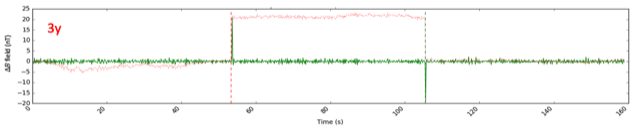
\includegraphics[width=\linewidth, height= 3 cm]{Images/1s1c3y}
%         \caption{for 3y and $C_x^-$ }
%         \label{fig:1s1c3y}
%     \end{subfigure}%
%     \begin{subfigure}{.5\linewidth}
%         \centering
%         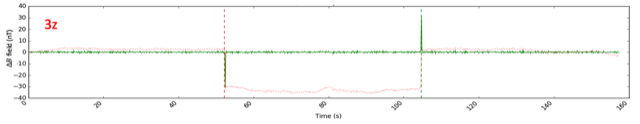
\includegraphics[width=\linewidth, height= 3 cm]{Images/1s1c3z}
%         \caption{for 3z and $C_x^-$}
%         \label{fig:1s1c3z}
%     \end{subfigure}\\[1ex]
%     \begin{subfigure}{.5\linewidth}
%         \centering
%         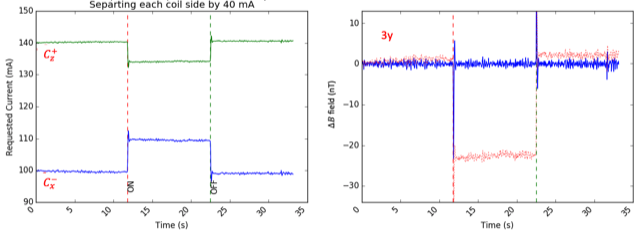
\includegraphics[width=\linewidth, height= 3 cm]{Images/1s2c3yc1c6}
%         \caption{for 3y, 3z, $C_x^-$ and $C_z^+$}
%         \label{fig:1s2c3yc1c6}
%     \end{subfigure}%
%         \begin{subfigure}{.5\linewidth}
%         \centering
%         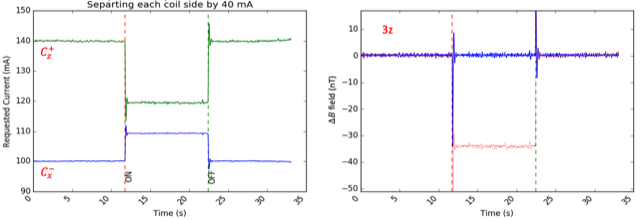
\includegraphics[width=\linewidth, height= 3 cm]{Images/1s2c3zc1c6}
%         \caption{for 3y, 3z, $C_x^-$ and $C_z^+$}
%         \label{fig:1s2c3zc1c6}
%     \end{subfigure}\\[1ex]
%     \begin{subfigure}{1\linewidth}
%         \centering
%         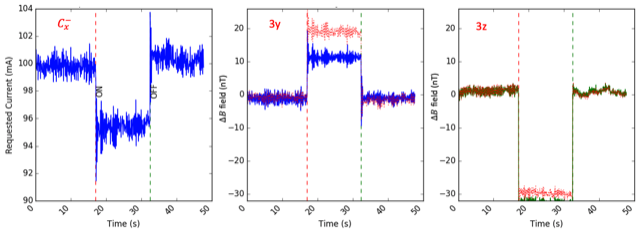
\includegraphics[width=\linewidth, height= 3 cm]{Images/2s1c3y3zc1}
%         \caption{for 3y, 3z and $C_x^-$ }
%         \label{fig:2s1c3y3zc1}
%     \end{subfigure}

%     \caption{The compensation effect due to individual coil. Vertical axis in Fig.~\ref{fig:1s1c3y} and in Fig~\ref{fig:1s1c3z} shows the $\Delta$ B found using Eq.~\ref{eq:del_B} over time for two different sensors where the green indicates $\Delta$ B due to compensation and the red indicates $\Delta$ B without compensation. Vertical axis in left of both Fig.~\ref{fig:1s2c3yc1c6} and  Fig.~\ref{fig:1s2c3zc1c6} indicates the coil current that has been sent to coils $C_x^-$ and $C_z^+$ to satblize 3y and 3z as shoen in right of those respectively. Initially both $C_x^-$ and $C_z^+$ were in the same level but for showing them together in the same figure they have been separated by some constant.  Vertical axis in left of Fig.~\ref{fig:2s1c3y3zc1} also indicates the current but only for $C_x^-$. Vertical axis in right of Fig.~\ref{fig:1s2c3yc1c6} and  Fig.~\ref{fig:1s2c3zc1c6} and in middle and right of Fig.~\ref{fig:2s1c3y3zc1} have the same description as in in Fig~\ref{fig:1s1c3z} }
%     \label{fig:1d}
% \end{figure}

% %\FloatBarrier
% The author in Ref.~\cite{bea} in Section \textcolor{blue}{7.2.3} of her PhD thesis claimed that more sensors than coils with some optimization give better compensation forming a non-square matrix which needs to be inverted for calculating the error using Eq.~\ref{eq:del_I}. 

The Moore--Penrose pseudo-inverse can be used for the inversion process. A tutorial review of the pseudo-inverse can be found in Ref.~\cite{pseudo}. The pseudo-inverse of a matrix can be computed using singular value decompostion (SVD). SVD is a factorization or diagonalization of a matrix. The matrix can be a real or complex square or rectangular matrix. The SVD~\cite{svd4,svd2,svd3} of a real rectangular matrix $\bm{M}$ with dimension $m \times n$ and $m>n$ is 
% \begin{equation}\label{eq:m}
%     \begin{split}
%         \bm{M} = \bm{U} \bm{\Sigma} \bm{V^T}
%               &=\begin{bmatrix} 
%                     \Sigma_{11} &  &  & 0 \\
%                     & . &  &  \\
%                     &   & . &  \\
%                     0 &  &  & \Sigma_{nn} \\
%                     \end{bmatrix}
%                 \begin{bmatrix} 
%                     \Sigma_{11} &  &  & 0 \\
%                      & . &  &  \\
%                      &   & . &  \\
%                      0 &  &  & \Sigma_{nn} \\
%                 \end{bmatrix}
%     \end{split}
% \end{equation}
\begin{equation}\label{eq:m}
    \bm{M} = \bm{U} \bm{\Sigma} \bm{V^T}
\end{equation}
% where, $\bm{U}\:\epsilon\:\mathbb{R}^{m \times m}$, $\bm{V^*}\:\epsilon\:\mathbb{R}^{n \times n}$ 
where, $\bm{U}$ and $\bm{V}$ are matrices with dimensions $m \times m$ and $n \times n$ respectively and $\bm{V^T}$ is the transpose of $\bm{V}$. $\bm{U}$ and $\bm{V^T}$ are composed of the left and right singular vectors representing the orthonormal eigenvectors of $\bm{M}\bm{M^T}$ and $\bm{M^T}\bm{M}$ respectively. $\bm{\Sigma}$ is a real non-negative diagonal matrix with the same dimension as  $\bm{M}$ and can be written as

\begin{equation}
\bm{\Sigma} = \begin{bmatrix} 
\Sigma_{11} &   &   & 0           \\
            & . &   &             \\
            &   & . &             \\
            &   &   & \Sigma_{nn} \\
            &   &   &             \\
          0 &   &   & 0          \\

 \end{bmatrix}
\end{equation}
where, $\Sigma_{11},..,\Sigma_{nn}$ are diagonal values of $\bm{\Sigma}$ with $\Sigma_{11}\gg...\; \Sigma_{nn}\geq0$. The positive square roots of the non-negative eigenvalues of $\bm{M^T}\bm{M}$ yield the $\Sigma_{ii}(i=1,..,n)$, and are called the singular values of $\bm{M}$. 

The point of SVD is that this is easy to invert because the transpose of an orthogonal matrix is equal to its inverse. That is $\bm{U^T}=\bm{U^{-1}}$ and $\bm{V^T}=\bm{V^{-1}}$ and
\begin{equation}\label{eq:sigma_inv}
\bm{\Sigma^{-1}=}\frac{1}{\bm{\Sigma}} = \begin{bmatrix} 
\frac{1}{\Sigma_{11}} &  &  &  &  &  & & &0\\
  & . &  &  & & & & &\\
  &   & . & & & & & &\\

0 &  &  & \frac{1}{\Sigma_{nn}} &  &  & & &0 \\
 \end{bmatrix}
\end{equation}

The pseudo-inverse of $\bm{M}$ will be then the inverse of $\bm{U}$, $\bm{\Sigma}$ and $\bm{V^T}$ and can be written as
\begin{equation}\label{eq:psMinv}
    \bm{M^{-1}} = \bm{V \Sigma^{-1} U^T}
\end{equation}


% ${\rm I\!R}$
%  \fig{Images/6c_U_Mcond26_p1368}{width = \textwidth}{Color map of $\bm{U}$ for transpose of $\bm{M}$ shown in Fig.~\ref{fig:m}. $\bm{U}$ is orthonormal eigenvectors of $\bm{M}\bm{M^T}$ in sensors$\times$sensors dimension for 12 sensors signals (nT). Red elements indicate positive values while blue elements indicate near zero values. \label{fig:6c_U}}{Color map of $\bm{U}$.}

 \fig{Images/V_30}{width =0.8\textwidth}{Color map of $\bm{\Sigma}$ for transpose of $\bm{M}$ shown in Fig.~\ref{fig:m}. $\bm{\Sigma}$ is positive square roots of the non-negative eigenvalues of $\bm{M^T}\bm{M}$ in sensors$\times$coils dimension for 12 sensors and 6 coils in nT/A. Red elements indicate positive values while blue elements indicate near zero values. \label{fig:v}}{Color map of $\bm{\Sigma}$}

%  \fig{Images/6c_Wt_Mcond26_p1368}{width = \textwidth}{Color map of $\bm{V^T}$ for transpose of $\bm{M}$ shown in Fig.~\ref{fig:m}. $\bm{V^T}$ is orthonormal eigenvectors of $\bm{M^T}\bm{M}$ in coils$\times$coils dimension for 6 coils currents (A). Red elements indicate positive values while blue elements indicate near zero values. \label{fig:6c_Vt}}{Color map of $\bm{V^T}$.}

% In earlier Section we have discussed a matrix $\bm{M}$ which is shown in Fig.~\ref{fig:m}. $\bm{M^T}$ is the transpose of that matrix. $\bm{M^T}$ has been decomposed via SVD in $\bm{U}$ , $\bm{\Sigma}$ and $\bm{V^T}$ which are shown in Fig.~\ref{fig:6c_U}, Fig.~\ref{fig:v} and Fig.~\ref{fig:6c_Vt} respectively. The $\bm{\Sigma}$ in Fig.~\ref{fig:v} shows that except diagonal values all are zero with the diagonal values are arranged from $\Sigma_{11}$ to $\Sigma_{nn}$ in a decreasing order each having non-negative values. 

% From those values the condition number of $\bm{M^T}$  can be found. The condition number of a matrix measures the change in the output for a small change in input. Large condition number indicates ill-conditioned matrix while small condition number indicates well-conditioned matrix. The condition number of $\bm{M^T}$ can be determined from the diagonal matrix $\bm{\Sigma}$ as 
%  \begin{equation}\label{eq:cond}
%      cond(\bm{M})=\frac{max(\Sigma_{ii})}{min(\Sigma_{ii})}
%  \end{equation}
 
% Using Eq.~(\ref{eq:cond}), the condition number of $\bm{M^T}$=5676/215=26.4 which indicates an ill-conditioned matrix.
Figure~\ref{fig:v} shows the diagonal matrix $\bm{\Sigma}$ for our measured $\bm{M}$. It is a diagonal with the singular values arranged from $\Sigma_{11}$ to $\Sigma_{66}$ in a decreasing order, each having a non-negative value. It is also noticeable that $\Sigma_{66}$ is very small compare to $\Sigma_{11}$. Since no. of coils ($c$) is less than no. of fluxgate sensors ($s$), it is easily thought of as represent modes of the coil set. If $\Sigma_{nn}<<\Sigma_{11}$ it means that mode corresponding to  $\Sigma_{nn}$ requires a much larger current in order to generate the same scale of magnetic field as for the $\Sigma_{11}$ mode. 


% \textcolor{red}{\bf{*************Need to Modify***************}}

% The reason can be explained by representing the Eq.~(\ref{eq:del_I}) in vector form.

% \begin{equation}\label{eq:del_I_pseudo}
%     \Delta\Vec{I} \approx\bm{M^{-1}}\Delta\Vec{B}=\bm{V \Sigma^{-1} U^T}\Delta\Vec{B}=\sum_{i=1}^{n}v_i\frac{u_i^T \Delta\Vec{B}}{ \Sigma_{ii}}
% \end{equation}
% where, rank of $\bm{M}$ is equal to the number of positive singular values. It is seen that $\Delta\Vec{I}$ for smaller $\Sigma_{ii}$ will be much larger compare to large $\Sigma_{ii}$ for same scale of field change $\Delta\Vec{B}$. In other-words, $\Delta\Vec{I}$ is dominated by right singular vectors $v_i$ due to small $\Sigma_{ii}$. The quantities $\frac{u_i^T \Delta\Vec{B}}{ \Sigma_{ii}}$ are the expansion coefficients for the basis vectors $v_i$. When these quantities are small in magnitude, the $\Delta\Vec{I}$ has very little contribution from $v_i$. But dividing by a small $\Sigma_{ii}$ greatly magnify the corresponding error component, $u_i^T \Delta\Vec{B}$, which in turn contributes a large multiple of the high-frequency information contained in $v_i$ to compute $\Delta\Vec{I}$. Due to this, the coil currents as well as magnetic field changes are dominated by high frequencies, which will be shown later in Fig.~\ref{fig:6c_pseudo_shield}. The above discussion is based on the similar problem faced while deblurring image which is explained nicely in Section~\textcolor{blue}{1.4} of Chapter~\textcolor{blue}{1} of Ref.~\cite{svd4}.

% \textcolor{red}{\bf{********************End************************}}

% The condition number of $\bm{M}$ being large therefore indicates that problematic modes exist which will have practically no control on the magnetic field.
In Section~\ref{sec:coil_config}, I analyze this effect further in both simulation and experiment. For now, I present the strategy of Ref.~\cite{bea} which I followed initially which involves matrix regularization.

Regularization methods help to reduce the dominance of singular vectors corresponding to small singualr values. Tikhonov regularization~\cite{tikhonov2013numerical,tikhonov_book,svd,svd3} is a commonly used regularization method which solves the problem by minimizing 

% The aim of the feedback algorithm is to make $||\Delta\Vec{B}-\bm{M}\Delta\Vec{I}||_2^2$ equal to zero. But making it zero will regenerate the original problem of larger $\Delta\Vec{I}$ for smaller $\Sigma_{ii}$ as explained above and by Eq.~(\ref{eq:del_I_pseudo}).
\begin{equation}\label{eq:tikhonov}
    ||\Delta\Vec{B}-\bm{M}\Delta\Vec{I}||_2^2+{\alpha}^2||\Delta\Vec{I}||_2^2
\end{equation}
where $||\cdot ||_2$ is the Euclidean norm rather than $||\Delta\Vec{B}-\bm{M}\Delta\Vec{I}||_2^2$ as done by the Moore--Penrose pseudo-inverse. Tikhonov regularization tries to make a compromise between $||\Delta\Vec{B}-\bm{M}\Delta\Vec{I}||_2^2$ and $||\Delta\Vec{I}||_2^2$ so that both of them are smaller. Tikhonov regularization makes that possible by introducing a filter $\alpha$ which sets the relative importance of the two terms. The filter $\alpha$ modifies the diagonal elements of $\bm{\Sigma^{-1}}$ from Eq.~(\ref{eq:psMinv}) as

\begin{equation}\label{eq:minvR}
    \frac{1}{\Sigma_{ii}} \rightarrow \frac{\Sigma_{ii}}{\Sigma_{ii}^2+\alpha^2} 
\end{equation}

In Ref.~\cite{bea}, Tikhonov regularization has been further modified by defining $\alpha=10^r$~nT/A where $r$ is called the regularization parameter. If  $r \rightarrow - \infty$, Eq.~(\ref{eq:minvR}) becomes the same as Eq.~(\ref{eq:sigma_inv}) indicating no regularization whereas $r \rightarrow + \infty$ results in $\bm{M^{-1}} \rightarrow 0$ resulting no control (as no changes to currents, and independent of $\Vec{B}$). Generally, $r$ should be of order $\mathbf{log}(\sigma_{d})$ in order for regularization to have its desired effect of making the diagonal values of $\bm{\Sigma^{-1}}$ more equal to one another. For example, suppose $\sigma_1$=100 and $\Sigma_{ii}$=1. The choice $\alpha$=10 results in

\begin{equation*}
    \frac{1}{\sigma_1} \rightarrow \frac{100}{100^2+10^2}=\frac{1}{101} 
\end{equation*}
\begin{equation*}
    \frac{1}{\Sigma_{ii}} \rightarrow \frac{1}{1^2+10^2}=\frac{1}{101} 
\end{equation*}
and, the singular values thereby become equalized.

The value of $r$ may be selected using several iterative methods. The obtained $r$ can be directly used in feedback algorithm to determine $\bm{M^{-1}}$. Because $\bm{M^{-1}}$ appears in the definition of the error in current (Eq.~(\ref{eq:del_I})), it has also an effect on the PI parameters. The PI parameters can be tuned in concert with $r$ by observing the effect on current response and this is studied further in Section~\ref{sec:r_pi}.


An iterative method has been discussed in the previous study~\cite{bea} to find $r$. I applied this concept to my system which will be discussed next.

% %\FloatBarrier

% \begin{equation}\label{eq:sigma}
%     \frac{1}{\sigma_d} \rightarrow \frac{\sigma_d}{\sigma_d^2+(10^r)^2}
% \end{equation}

% So, the Eq.~(\ref{eq:psMinv}) will be modified due to the modified form of Tikhonov regularization as
% \begin{equation}\label{eq:minvR}
%     \bm{M^{-1}}(r) = \bm{V}\begin{pmatrix} 
% \frac{\sigma_1}{\sigma_1^2+(10^r)^2} & 0 \\
% 0 & \frac{\sigma_d}{\sigma_d^2+(10^r)^2}
% \end{pmatrix} \bm{U^T}
% \end{equation}



% \fig{Images/v}{width = \textwidth}{Color map of $\Sigma$ for a test $\bm{M}$ found using Python programming language. Horizontal axis indicates the various coils, which are counted using the index $c$. Vertical axis indicates the various sensors, which are counted using the index $s$. Red elements indicate positive values while blue elements indicate near zero values. \label{fig:v}}{Color map of $\Sigma$}

% %\FloatBarrier

% The problem can visualized from Fig.~\ref{fig:m} where for example X-(1) has negligible sensitivity for 3x which means that particular matrix element (in nT/A) is very small. So, the pseudo-inverse of $\bm{M}$ using Eq.~\ref{eq:psMinv} will produce very large element (in A/nT) which means that the amount of current will be huge there which will make the prototype unstable. To minimize the effect, the matrix must be regularized which means that all ill-conditioned places must be replaced  by well-conditioned ones.  



\subsection{Regularization by Random Fluctuation}\label{sec:mont}

The method of a previous study~\cite{bea} was adapted for my prototype to determine a value of $r$ by studying its effect on the ability to cancel random field fluctuations without generating unacceptably large current fluctuations.

For this method, sets of reasonable random magnetic fields ($B_s^{\text{rand}}$) are generated according to the normal distribution and standard deviation of 1.5~nT. As in Ref.~\cite{bea}, the reasonable value for the standard deviation was determined by the scale of the fluctuations seen from second to second by the sensor array (presented in Fig.~\ref{fig:hist}). The exact value of the standard deviation will turn out to be unimportant in the way Ref.~\cite{bea} finally deduces $r$ using normalized field and current fluctuations.

Using the setpoint as zero, according to Eq.~(\ref{eq:del_B}) the change in the sensed field is  
\begin{equation}\label{eq:del_Bs}
    \Delta B_s^{\text{sim}} = 0 - B_s^{\text{rand}}=-B_s^{\text{rand}}
\end{equation}
The array of the current errors  as function of $r$ due to the the change in field $\Delta B_s^{\text{sim}}$ is then calculated using the regularized pseudo-inverse using Eq.~(\ref{eq:del_I}) as
\begin{equation}\label{eq:del_Is}
    \Delta I_c^{\text{sim}}(r) =\sum_{s=1}^{12} M^{-1}_{cs}(r) \Delta B_s^{\text{sim}}=\sum_{s=1}^{12} M^{-1}_{cs}(r) (-B_s^{\text{rand}})
\end{equation}
To estimate the overall current response from the array, the root mean square (RMS) of $\Delta I_c^{\text{sim}}(r)$ is calculated as
\begin{equation}\label{eq:delta_Isim_rms}
     \Delta I_{\text{RMS}}^{\text{sim}}(r)= \sqrt{\frac{1}{6}\sum_{c=1}^6 (\Delta I_c^{\text{sim}}(r))^2}~\text{.}
\end{equation}
This is calculated as a function of $r$ for different sets of $B_s^{\text{rand}}$ (Fig.~\ref{fig:Isim}). With the increase of $r$, the current fluctuations $\Delta I_{\text{RMS}}^{\text{sim}}$ vanish as expected.


% $ \Delta I_{\text{RMS}}^{\text{sim}}(r)$ as indicated by vertical axis over $r$ as indicated by horizontal axis has been shown for 30 different sets of $B_s^{\text{rand}}$. The distribution $B_s^{\text{rand}}$ is randomly chosen with center of distribution and standard deviation is discussed earlier. 

\fig{Images/6c_I}{width=0.8\textwidth}{The effect of $r$ on the coil currents for 30 different sets of $B_s^{\text{rand}}$ generated according to the normal distribution with a central value of 0 and standard deviation 1.5 nT. The horizontal axis represents $r$ while the vertical axis shows $\Delta I_{\text{RMS}}^{\text{sim}}$. \label{fig:Isim}}{The effect of $r$ on the coil currents.}

%\FloatBarrier
The field produced by $ \Delta I_c^{\text{sim}}$ can be calculated using Eq.~(\ref{eq:B_coils}). The total field at each sensor $s$ will be the superposition of $B_s^{\text{rand}}$ and the response produced by $ \Delta I_c^{\text{sim}}(r)$ 
\begin{equation}\label{eq:B_coils-sim}
    B_s^{\text{sim}}(r) =\sum_{c=1}^6 M_{sc} \Delta I_c^{\text{sim}}(r) + B_s^{\text{rand}}
\end{equation}
For a perfectly compensated system, the field produced by $ \Delta I_c^{\text{sim}}$ would equal $- B_s^{\text{rand}}$ which in turn would make the $B_s^{\text{sim}}(r)$ in Eq.~(\ref{eq:B_coils-sim}) identically zero. In practice, this is rarely the case. To quantify the effectiveness of the compensation,  the ratio of RMS of $B_s^{\text{sim}}(r)$ to the RMS of $B_s^{\text{rand}}$ is calculated as
\begin{equation}\label{eq:fluc}
    F(r)=\frac{\sqrt{\frac{1}{12} \sum_{s=1}^{12} (B_s^{\text{sim}}(r))^2}}{\sqrt{\frac{1}{12} \sum_{s=1}^{12} (B_s^{\text{rand}}(r))^2}}
\end{equation}
The function $F(r)$ would be zero for a perfectly compensated system and unity for an uncompensated system. In Ref.~\cite{bea}, $F(r)$ is called the ``remaining noise". The values of $F(r)$ shown in Fig.~\ref{fig:fluc-sim} are for the same sets of $B_s^{\text{rand}}$ used in Fig.~\ref{fig:Isim}. It is seen that with the increase of $r$, the field produced by $\Delta I_c^{\text{sim}}$ to compensate $B_s^{\text{rand}}$  are increasing resulting in more field fluctuations. It is also noticeable that the system cannot be fully compensated because $F(r)$ never goes to zero. The lowest $F(r)$ is 0.45, indicating the system will not be terribly successful at correcting random fluctuations. We think this is mainly due to the limited coil design used for this prototype, which was designed instead to focus on issues in multi-dimensional PI control.

\fig{Images/6c_f}{width =0.8\textwidth}{The effect of $r$ on the effectiveness of field compensation indicated by the remaining fluctuation $F(r)$. The different curves indicate 30 different sets of $B_s^{\text{rand}}$. \label{fig:fluc-sim}}{The effect of $r$ on remaining fluctuations.}

%\FloatBarrier
It is seen from Figs.~\ref{fig:Isim} and \ref{fig:fluc-sim} that with the increase of $r$, current fluctuations decrease but field fluctuations increase. Ref.~\cite{bea} suggested a compromise between them be struck to determine the value of $r$, $\it i.e.$ that reducing current fluctuations ($r \rightarrow + \infty$) be traded off against reducing magnetic field fluctuations ($r \rightarrow - \infty$). To decide the value of $r$, $\Delta I_{\text{RMS}}^{\text{sim}}(r)$ and $F(r)$ were normalized to make their range extend from 0 to 1 using

\begin{align}
    \overline{\Delta I_{\text{RMS}}^{\text{sim}}}(r) &= \frac{\Delta I_{\text{RMS}}^{\text{sim}}(r)}{\Delta I_{\text{RMS}}^{\text{sim}}(r\rightarrow - \infty)} \;\mathrm{,\;and}\label{eq:Inorm}\\
    \overline{F}(r) &= \frac{F(r)- F(r\rightarrow - \infty)}{F(r\rightarrow \infty)- F(r\rightarrow - \infty)}~\text{.}\label{eq:flucNorm}
\end{align}

\fig{Images/6c_I-fluc2}{width =0.8\textwidth}{The normalized $\overline{\Delta I_{\text{RMS}}^{\text{sim}}}$ and $\overline{F}$ for 30 sets of $B_s^{\text{rand}}$. The red line indicates the 0.5 level.\label{fig:I-fluc}}{The effect of $r$ on normalized current and remaining fluctuations.}

%\FloatBarrier
The effect of $r$ on $\overline{\Delta I_{\text{RMS}}^{\text{sim}}}$ and $\overline{F}$ is shown in Fig.~\ref{fig:I-fluc}. With an increase in $r$, $\overline{\Delta I_{\text{RMS}}^{\text{sim}}}$ decreases and $\overline{F}$ increases as expected from the discussion earlier.
Two values of $r$ were then found for each $B_s^{\text{rand}}$ by alternatively setting $r$ on $\overline{\Delta I_{\text{RMS}}^{\text{sim}}(r)}$ and $\overline{F(r)}$=0.5. This is indicated schematically by the horizontal line in Fig.~\ref{fig:I-fluc}. The values of $r$ so determined are averaged and in turn the averages are averaged over a large number of $B_s^{\text{rand}}$ ($=30$). The optimized $r$ in the example of Fig.~\ref{fig:I-fluc} is found to be 2.87.

The calculation to find $r$ gives insight about the effect of regularization on current and field fluctuations, resulting in a compromise that adequately reduces both. With $r$ in hand, $\bm{M^{-1}}$ and thus the current error may be determined which is used in the PI algorithm.

\section{Tuning of PI Parameters}\label{sec:tune}
This section describes the tuning of the proportional gain $k_c^p$ and integral reset $k_c^i$ terms appearing in Eq.~(\ref{eq:I}) to compensate the changes in magnetic fields measured by the fluxgate sensors.

% According to the type of system and the way the control loop for a particular system has been chosen, 
The PI parameters can be tuned using various methods~\cite{tuning}. A common tuning method is Ziegler-Nichols closed tuning method~\cite{tuning_ZN}. I usually used this method as an initial guess for the PI parameters. In the Ziegler-Nichols method, $k_c^i$ is first set to zero and $k_c^p$ is increased until the currents in the coils start oscillating. The $k_c^p$ value for which the current in the coils start oscillating is denoted the ultimate gain $G_{u}$ and the period of the oscillation is denoted the ultimate oscillation period $T_u$. The the value of $k_c^p$ and $k_c^i$ are then determined based on the PI row of Table~\ref{table:tuning}. Table~\ref{table:tuning} is a modified version of the Table~\textcolor{blue}{4} in Ref.~\cite{tuning_formula} where the formula for integral time $T_i=T_u/1.2$ has been used. 

\begin{table} [htb!]
    \centering
    \begin{tabular} { |c|c|c|c|c|c|} 
        \hline
        Controller & Gain ($k_c^p$) & Reset ($k_c^i$)\\
        \hline\hline
         P & 0.5 $G_u$ & 0 \\ 
        \hline
         PI & 0.45 $G_u$ & $\left(\frac{\text{0.54} G_u}{T_u}\right)\Delta t$ \\ 
        \hline
    \end{tabular}
    % \vspace{4mm}
    \caption{Ziegler-Nichols tuning method for P and PI controllers.}\label{table:tuning}
\end{table}

%\FloatBarrier
% In Ref.~\cite{tuning_formula}, it is also mentioned that $k_c^i=(k_c^p/T_i)$ which for our case will be $k_c^i=(k_c^p/T_i)\Delta t$, where, $\Delta t$ is the time difference between two consecutive feedback loop. So, $k_c^i$ will be
% \begin{equation}
%     k_c^i=\left(\frac{k_c^p}{T_u/1.2}\right)\Delta t=\left(\frac{1.2\times0.45 G_u}{T_u}\right)\Delta t=\left(\frac{0.54 G_u}{T_u}\right)\Delta t
% \end{equation}

The quantity $\Delta t$ in Table~\ref{table:tuning} is the time to complete one feedback loop iteration.

\fig{Images/p134c1}{width =0.9\textwidth}{Zoomed current behaviour in coil $C_x^+$ with $k_c^p$ =1.34 and $k_c^i$=0. Vertical axis represent the currents in coil $C_x^+$ with initial current being 100 mA. For position of the coil see Fig.~\ref{fig:coil}. \label{fig:tuning}}{Zoomed current behaviour in coil $C_x^+$.}
% in response to the perturbation coils
%\FloatBarrier
Figure~\ref{fig:tuning} shows the first step in the tuning process. For simplicity, zoomed version of the current in coil $C_x^+$ is shown only. At $k_c^p$=1.34 and $k_c^i$=0, the current in the coils oscillates allowing us to identify $G_u$=1.34.  The ultimate period is $T_u$=0.287~s. Now, according to Table~\ref{table:tuning}, the proportional gain and integral reset are

\begin{equation}
    k_c^p=0.45\times1.34=0.60\;\;\text{and}\;\; k_c^i=\left(\frac{0.54 \times1.34}{0.287}\right)\times0.146=0.37
\end{equation}
They can be further tuned for the individual coil currents if necessary but we elected not to study this. In general, we treated them as free parameters and studied the impact of changing them on system response. More about PI tuning will be discussed in the next chapter with compensation results.



% \doublefig{Images/p97}{width =\textwidth,height=8cm}{at $k_c^p$=0.97. \label{fig:tuningNmod}}{Images/p97mod}{width = \textwidth,height=8cm}{$k_c^p$=0.97 with zoomed $C_y^-$.\label{fig:tuningMod}}{{The current behaviour in all six coils with $k_c^p$ =0.97 and $k_c^i$=0. Vertical axes represent the currents in all six coils having different colors. The 'ON' and 'OFF' vertical dashed lines indicate the time of the perturbation coil being turned 'ON' and 'OFF' respectively. Both the figures are same except the current in $C_z^+$ coil has been zoomed in left figure.  } \label{fig:tuning}}{Tuning by observing coil currents}



% Moreover, to double check, the experimentally obtained $\bm{M}$ has been compared with a simulation done using finite element analysis (FEA) via Opera 3D software as shown in Fig.\ref{fig:Mdiff}.


%  \fig{Images/Mdiff}{width =  \textwidth}{Comparison of Experimental M with Simulation \label{fig:Mdiff}}
 
 
% 

% Fig.\ref{fig:bt} shows the compensation over time with applied perturbation. \newpage
%\FloatBarrier




\section{Quantitative Measures of Magnetic Compensation Performance\label{sec:metrics}}
% For every system, there are some metrics, which quantitatively determine the system's performance. The success of the prototype has been claimed similarly. 
I considered four main three metrics, which are based on previous studies of others~\cite{bea,lins,rawlik}. They are:

\begin{enumerate}
    \item Condition Number,
    \item Reduction of Magnetic Field Fluctuation and PI Behavior upon Stimulus, and
    \item Allan Deviations and Shielding Factor
\end{enumerate}

Each will be described. In Chapter~\ref{ch:quantification}, I will use these definitions and study them under various conditions.

\subsection{Condition Number}

% The condition number of a matrix measures the change in the output for a small change in input. Large condition number indicates ill-conditioned matrix while small condition number indicates well-conditioned matrix. 

The condition number of the matrix $\bm{M}$ can be determined from the diagonal matrix $\bm{\Sigma}$ as 
 \begin{equation}\label{eq:cond}
     \mathrm{cond}(\bm{M})=\frac{\mathrm{max}(\Sigma_{ii})}{\mathrm{min}(\Sigma_{ii})}=\frac{\Sigma_{11}}{\Sigma_{nn}}
 \end{equation}

The condition number of a matrix is $\geq$1 by definition. Low condition number indicates a well-conditioned matrix while large indicates an ill-conditioned matrix. Sample diagonal elements $\Sigma_{ii}$ were shown in Fig.~\ref{fig:v}. Using Eq.~(\ref{eq:cond}),  $\mathrm{cond}(\bm{M})=5448.0/184.0=29.61$ which indicates an ill-conditioned matrix. 
% So having a very small $\Sigma_{ii}$ indicates an ill-conditioned matrix. Larger condition number also indicates that the $\Delta\Vec{I}$ is very sensitive to perturbation and rounding errors $u_n^T \Delta\Vec{B}$ (see Eq.~(\ref{eq:del_I_pseudo})).
% The condition number of $\bm{M}$ being large therefore indicates that problematic modes exist which will have practically no control on the magnetic field.

% The condition number can be influenced by the dimension of a matrix. But, the change in condition number in case of  well-conditioned matrix is incomparably smaller than that in a ill-conditioned matrix~\cite{cond_m_size}. However, there is no upper bound that indicates the limit of well-conditioned matrix. So, there is no definite answer about how small is considered as well-conditioned matrix. so that compensating a certain scale of change in magnetic field requires less change in current and also the compensation system does not loose its effect on all the sensors while making the condition number less.

In testing the active compensation system, the goal is to have matrix condition number as close to 1 as possible. If $\Sigma_{nn}$ is small ({\it e.g.} zero), it means that the $B_s$ never change no matter what the current for that mode. Consequently, on inverting, large currents are driven for that mode with practically no change in the $B_s$. Tikhonov regularization is one method of reducing the condition number closer to 1 but later I discovered that designing a well-conditioned system is a better method. A comparison of those methods is discussed in Section~\ref{sec:coil_config}.

% The main aim is to make the prototype well-conditioned by determining the best compromise between current and field fluctuations which will lead us to the optimized $r$. It has been also explored to determine whether the optimized $r$ is giving the best result or not. If not, additional parameters have been tuned to get the best possible result.

\subsection{Reduction of Magnetic Field Fluctuation and PI Behavior upon Stimulus}

% Active magnetic field compensation come into play in the first place to make the surrounding magnetic fluctuations as small as possible. So, prototype response for magnetic fluctuations has been studied in terms of its capabilities as reduction or amplification. We have already shown in Fig.~\ref{fig:fluc-sim} that the lowest remaining fluctuations due to several random fluctuations is 0.45. Ideally, the remaining fluctuations should be zero. The system is completely unsuccessful if the remaining fluctuation is found to be 1. Our goal for the prototype is to get remaining fluctuation at least 0.5.

For active magnetic compensation, the measured field by the fluxgate sensors $B_s^n(\text{meas})$ is the superposition of the the uncompensated field and the field created by the compensation coils $B_s^n(\text{coils})$ at the sensor positions for $n$=(1,...,N) number of measurements. The uncompensated field is thus estimated to be the the magnetic field without the compensation effect by subtracting the $B_s^n(\text{coils})$ from the $B_s^n(\text{meas})$ {\it i.e.}
% The magnetic field without the compensation effect referred to as the uncompensated magnetic field. It is estimated using 
\begin{equation}\label{eq:Buncomp}
     B_s^n(\text{uncomp})=B_s^n(\text{meas})- B_s^n(\text{coils})
\end{equation}
where, $B_s^n(\text{coils})$ is determined using Eq.~(\ref{eq:B_coils}).



\fig{Images/bt-mod}{width=0.9\textwidth}{Magnetic field reduction at some of the sensors closer to the perturbation coil and the central position. Color curves: measured field change $=B_s^n(\text{meas})$. Red curves: extracted uncompensated field change $ B_s^n(\text{uncomp})$. Vertical dashed lines indicate the time of the perturbation coil being turned on and off.\label{fig:bt_mod}}{Magnetic field reduction at some of the sensor positions.} 

The PI feedback and control system can be tested by its response to a step the perturbation coil current. This can also be studied by monitoring the central sensors within the passive magnetic shielding system. An example of this is shown in Fig.~\ref{fig:bt_mod} where both $B_s^n(\text{meas})$ and $B_s^n(\text{uncomp})$ are shown.  The active compensation reduces the effect of the perturbation coil current in the sensors. The central sensor's response is also compensated somewhat. I expect the limitation in the correction is due to limitations in the coil design. 

% position and to some levels in other positions indicated by blue, green and cyan colors. Moreover, the last one named 'center-Z' predicts the response in the center of the prototype in $z$ axis without actually being in the feedback loop and there is also improvement in terms of step response level. We are considering the good results if the system response time is fastest without any overshoot and also reduces the step response levels as much as possible. The results are considered bad if the there is very slow response of the system.


%\FloatBarrier
The RMS current change and RMS field change for both the measurement and in the uncompensated case can be determined experimentally under application of perturbation coil current.

% \begin{align}
%     \Delta I_c^{\text{exp}}(r) &= \sum_{s=1}^{12} M^{-1}_{cs}(r) (-B_{\text{uncomp}}(r))\label{eq:del_Is_exp}\\
%      \Delta I_{\text{RMS}}^{\text{exp}}(r) &= \sqrt{\frac{1}{6}\sum_{c=1}^6 (\Delta I_c^{\text{exp}}(r))^2}\label{eq:delta_Iexp_rms}
% \end{align}
% Furthermore, to find 

The remaining fluctuations can also be quantified experimentally
\begin{equation}\label{eq:fluc_exp}
   F(\mathrm{exp})=\frac{\sqrt{\frac{1}{12} \sum_{s=1}^{12} \Delta B_s(\text{meas})^2}}{\sqrt{\frac{1}{12} \sum_{s=1}^{12} (\Delta B_s(\text{uncomp})^2}}
\end{equation}
where, $\Delta B_s(\text{meas})$ and $\Delta B_s(\text{uncomp})$ measured step changes in the measured and uncompensated magnetic fields, respectively, under application of the perturbation coil current.

\fig{Images/mont_exp}{width =0.9\textwidth}{Experimentally determined effect of $r$ on (left) RMS current change  and (right) remaining field fluctuations $F(\mathrm{exp})$ for $k_c^p=1.0$ and $k_c^i=0.0$. Fluxgates were located at positions 1, 2 and 7 in this study, and 100~mA current was supplied in the perturbation coil. \label{fig:mont_comp}}{The effect of $r$ for experimental setup.}


An example of the effect of $r$ on the RMS current change  and $F(\mathrm{exp})$ for a particular perturbation coil current step is shown in Fig.~\ref{fig:mont_comp}. It is seen that around 100~mA RMS of current array is required to compensate the perturbation
which eventually vanishes with $r$ increment as expected (Fig.~\ref{fig:mont_comp}\textcolor{blue}{(a)}). Furthermore, field fluctuations are reduced to $50\%$ of their uncompensated values.






 
 \subsection{Allan Deviations and Shielding Factors}
 
The Allan standard deviation \cite{allan} is used to test the time stability of clocks, amplifiers and oscillators. The same concept can be applied to time series of the magnetic field measurements. In this case, the Allan standard deviation is defined as~\cite{bea}
\begin{equation}\label{eq:adev}
    \sigma_{Adev} (\tau)=\sqrt{\frac{1}{2(N-1)}\sum_{l=1}^{N-1} \left(\overline{B_{l+1}}(\tau)-\overline{B_l}(\tau)\right)^2}
\end{equation}
where, $\overline{B_l}(\tau)$ is the average magnetic field for a subset $l$ over integration time $\tau$ and $\tau = \frac{T}{N}$ with $T$ the total measurement time, and $N$ the total number of subsets. The $\sigma_{Adev}$'s dependence on $\tau$: $\sigma_{Adev}\approx$1/$\sqrt{\tau}$ indicates the data are statistically distributed with the same mean in the values, $\sigma_{Adev}\approx \sqrt{\tau}$ indicates a random walk in the values, and $\sigma_{Adev}\approx \tau$ indicates a linear drift~\cite{allan_tau}. 

\fig{Images/sf_b}{width =0.9\textwidth}{ (top) Field fluctuations $\Delta B$ for sensor 8x with the feedback switched off, (bottom) corresponding Allan standard deviation. Red horizontal lines represent $\overline{B_l}(\tau)$ for 8 subsets over integration time $\tau=128$~s separated by the vertical dashed lines. \label{fig:sf_mod}}{The Allan deviation.}


An example of the process of calculating the Allan deviation for magnetic field data is shown in Fig.~\ref{fig:sf_mod}. In this example, the feedback system was switched off. The top panel in Fig.~\ref{fig:sf_mod} demonstrates the division of the time series into eight $\tau$: 128~s-long subsets. The red line indicate the average of each subset $B_l^{\tau}$. The Allan deviation formula (Eq.~(\ref{eq:adev})) is applied to these averages to arrive at the data point at $\tau=128$~s in the bottom panel's Allan deviation plot in Fig.~\ref{fig:sf_mod}.  It is seen that $\sigma_{Adev}$ rises by about one decade for every two decades in $\tau$. This indicates that $\sigma_{Adev}\approx \sqrt{\tau}$ which refers random walk in the field values when there is no compensation system is running. The largest integration time over which $\sigma_{Adev}$ can be determined is $\tau_{\text{max}}=T/2$ as can be seen from the horizontal axes of Fig.~\ref{fig:sf_mod}. The total number of subsets for $\tau_{\text{max}}$ is $N = \frac{T}{\tau_{\text{max}}}=\frac{T}{T/2}=2$. 

% However, $\sigma_{Adev}(\tau_{\text{max}})$ is statistically insignificant while comparing the allan deviation measurements (measured and uncompensated), since there is only one subtraction in Eq.~(\ref{eq:adev}) and thus $\sigma_{Adev}(\tau_{\text{max}})$ will be neglected in such case.


% \fig{Images/sf_mod}{width =\textwidth,height=12cm}{The Allan deviation (top) and shielding factor (bottom) for signals from some fluxgate sensors. Top vertical axis indicates the Allan deviation while bottom indicates shielding factor. Horizontal axis indicates the integration time. The different colors in top and bottom have been discussed in text.  \label{fig:sf_mod}}{The Allan deviation.}



The goal of the active compensation system is to reduce the the Allan deviation to be less than the Allan deviation of the uncompensated magnetic field. This would indicate that the magnetic field is more stable with compensation than without. The shielding factor~\cite{bea} is defined as the ratio of Alllan deviations.
\begin{equation}\label{eq:sf}
    \text{sf} (\tau)=\frac{\sigma_{\text{Adev}}^{\text{uncomp}}(\tau)}{\sigma_{\text{Adev}}^{\text{meas}}(\tau)}
\end{equation}
The shielding factor $\text{sf} (\tau)>1$ indicates that the magnetic environment was improved. $\sigma_{Adev}(\tau_{\text{max}})$ will be neglected for calculating the $\text{sf} (\tau)$ . Because $\sigma_{Adev}(\tau_{\text{max}})$ is statistically insignificant while comparing the Allan deviation measurements since there is only one subtraction in Eq.~(\ref{eq:adev}). The shielding factor is discussed further in Section~\ref{sec:adev_res}.
 

%\fig{Images/sf}{width = 0.5 \textwidth}{Allan Deviation and Shielding Factor \label{fig:sf}}
 
 
 
